A Interface de Periféricos Serial, ou SPI (\emph{Serial Peripheral Interface}) é um dispositivo usado para a transmissão e recepção serial de dados. Sendo uma comunicação síncrona, a SPI necessita de uma fonte de clock de referência para se estabelecer, além de um sinal de \emph{chip select}, ou \textbf{CS}, para ativar a recepção de dados no dispositivo receptor. Deste modo esta comunicação requer no minimo três vias de transmissão, sendo que a comunicação em cada barramento é unidirecional.

\section{Padrão da Comunicação}

A comunicação SPI possui a maior taxa de transmissão, ou \emph{baud-rate}, dentre os demais protocolos de comunicação usados em microcontroladores, podendo chegar a até a 66Mpbs em periféricos com o AT45BD0100D da Adesto. O que possibilita um  \emph{baud-rate} tão elevado é o fato de que nesta comunicação a recepção e a transmissão de dados é feita separadamente e de forma direta, sem a necessidade de se transmitir bits de inicio ou termino de transmissão, e ainda de modo que o controle da transmissão é realizado pelo sinal CS (Chip Select) e pelo sinal  CLK (Clock).  A figura \ref{fig:SPI} apresenta o padrão de uma comunicação SPI.

\begin{figure}[H]
	\centering
	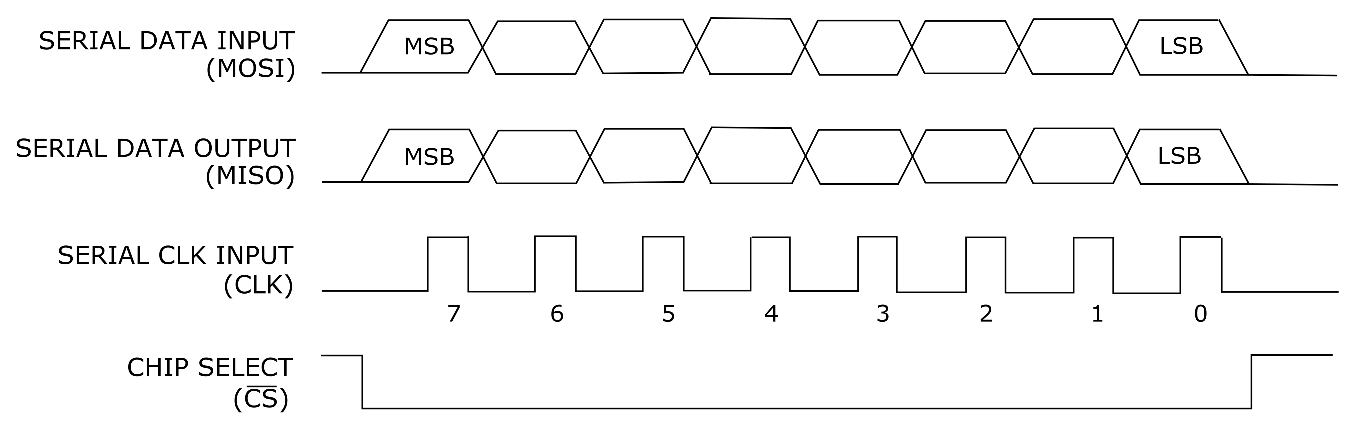
\includegraphics[width=1\textwidth] {figuras/PadraoSPI.eps}
	\caption{Padrão de Comunicação SPI}
	\label{fig:SPI}
\end{figure}

Para transmitir um dado de um dispositivo \textbf{Mestre} para um \textbf{Escravo} é necessário que o \textbf{Mestre} ative o sinal de CS do \textbf{Escravo} e forneça a ele o sinal de clock de referência. Em seguida bit a bit deve ser transmitido pela porta MOSI \emph{Master Output - Slave Input} de ambos os dispositivos. 

Quando for necessário transmitir um dado de um  \textbf{Escravo} para um \textbf{Mestre}, novamente o \textbf{Mestre} deve ativar o sinal de CS do  \textbf{Escravo} e fornecer a ele o sinal de clock de referência, porém o dado será transmitido bit a bit pela porta MISO \emph{Master Input - Slave Output} de ambos os dispositivos. 

\begin{figure}[H]
	\centering
	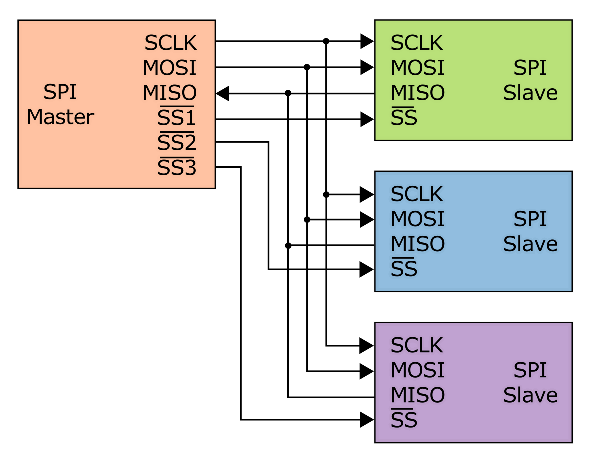
\includegraphics[width=0.6\textwidth] {figuras/BarramentoSPI.eps}
	\caption{Diagrama de Comunicação SPI - Vários Escravos}
	\label{fig:SPIDiagrama}
\end{figure}

A figura  \ref{fig:SPIDiagrama} apresenta um diagrama básico de uma comunicação entre \textbf{Mestre} e vários \textbf{Escravos} através dos barramentos de dados e de clock em comum.  

\section{SPI do TM4C1294NCPDT}

No Tiva - TM4C1294NCPDT a comunicação SPI se dá através do Interface Serial Quad Sincrona (\emph{Quad Synchronous Serial Interface}), ou QSSI. Há 4 módulos QSSI no Tiva, todos capazes de transmitir dados no modo Advanced, Bi-SSI e Quad-SSI.

No modo de transmissão Bi-SSI, dois pinos de dados são ativados para receber ou transmitir; SSInXDAT0 e o SSInXDAT1. Já no modo de transmissão Quad-SSI, quatro pinos são ativados para receber ou transmitir dados; SSInXDAT0, SSInXDAT1, SSInXDAT2 e SSInXDAT4. 

No modo de transmissão Advanced, a transmissão se realiza de modo que ao transmitir um dado por um pino, o outro pino fica impossibilitado de receber, e vice-versa.

A forma de transmissão dos módulos QSSI podem ser alterados entre os formatos \emph{Texas Instruments synchronous serial} e \emph{Freescale SPI}. Logo para transmitir em modo SPI basta somente selecionar o modo \emph{Freescale SPI}, podendo utilizar tanto o modo de transmissão Bi- ou  Quad-SSI.

No modo de comunicação SPI, tem-se um \emph{baud rate} máximo de 2MHz e uma FIFO para transmissão e outra para recepção ambas com capacidade de 16x8 bits. É possível alternar a fonte de clock de referência da transmissão entre o clock padrão do sistema (SYSCLK) e o clock alternativo (ALTCLK), contando ainda com um divisor de clock de 8 bits, que possibilita dividir o clock de 1 até 254 vezes.  

Como é comum na comunicação SPI o Tiva possui portas para transmissão, recepção e clock exclusiva para cada  módulo de comunicação. A tabela \ref{tab:CanaisSPI} apresenta as referidas portas para comunicação SPI.

\begin{table}[H]
	\centering
	\caption{Canais do SPI - Tiva TM4C1294NCPDT \cite{DATASHEET_TIVA} }
	\label{tab:CanaisSPI}
	\begin{tabular}{|c|c|c|c|l|}
		\rowcolor[HTML]{000000} 
		{\color[HTML]{FFFFFF} Pino}  & {\color[HTML]{FFFFFF} Mux/Função} & {\color[HTML]{FFFFFF} Tipo} & {\color[HTML]{FFFFFF} Buffer} & {\color[HTML]{FFFFFF} Descrição}  \\
		\hline
		SSI0CLK   & PA2 (15) & I/O & TTL & SPI Módulo 0, sinal de clock   \\
		\hline
		SSI0XDAT0 & PA4 (15) & I/O & TTL & SPI Módulo 0, MISO \\
		\hline
		SSI0XDAT1 & PA5 (15) & I/O & TTL & SPI Módulo 0, MOSI \\
		\hline
		SSI1CLK   & PB5 (15) & I/O & TTL & SPI Módulo 1, sinal de clock   \\
		\hline
		SSI1XDAT0 & PE4 (15) & I/O & TTL & SPI Módulo 1, MISO  \\
		\hline
		SSI1XDAT1 & PE5 (15) & I/O & TTL & SPI Módulo 1, MOSI  \\
		\hline
		SSI2CLK   & PB5 (15) & I/O & TTL & SPI Módulo 2, sinal de clock   \\
		\hline
		SSI2XDAT0 & PD1 (15) & I/O & TTL & SPI Módulo 2, MISO  \\
		\hline
		SSI2XDAT1 & PD0 (15) & I/O & TTL & SPI Módulo 2, MOSI  \\
		\hline
		SSI3CLK   & PQ0 (14) & I/O & TTL & SPI Módulo 3, sinal de clock   \\
		          & PF3 (14) &     &     &                                \\
		\hline
		SSI3XDAT0 & PQ2 (14) & I/O & TTL & SPI Módulo 3, MISO  \\
		          & PF1 (14) &     &     &                     \\
		\hline
		SSI3XDAT1 & PQ3 (14) & I/O & TTL & SPI Módulo 3, MOSI  \\
		          & PF0 (14) &     &     &                     \\
		\hline
	\end{tabular}
\end{table}


\section{Na TivaWare}

As principais funções de configuração e utilização da SPI pela TivaWare são listadas a seguir. São utilizadas as funções da SSI, porém são destacadas somente as funções que se referem à SPI.

\begin{lstlisting}[style=funcao]
	void SSIConfigSetExpClk(uint32_t ui32Base,
							uint32_t ui32SSIClk,
							uint32_t ui32Protocol,
							uint32_t ui32Mode,
							uint32_t ui32BitRate,
							uint32_t ui32DataWidth)
\end{lstlisting}

Configura a interface serial síncrona.

\begin{description}
	\item [\ttbu{ui32Base}]\hfill \\
	Base da interface serial síncrona a ser configurada. Normalmente \textbf{SSI\emph{k}\_BASE}, onde \textbf{\emph{k}} é a letra identificadora do gerador.
	
	\item [\ttbu{ui32SSIClk}]\hfill \\
	Frequência do clock da comunicação.
	
	\item [\ttbu{ui32Protocol}]\hfill \\
	Protocolo utilizado. No caso da SPI, é utilizado o valor \textbf{SSI\_FRF\_MOTO\_MODE\_\emph{k}}, onde \textbf{\emph{k}} assume valores de 0 a 3.
	
	\item [\ttbu{ui32Mode}]\hfill \\
	Valor do modo de operação. Definido no formato \textbf{SSI\_MODE\_\emph{k}}, onde \textbf{\emph{k}} assume os valores:
	\begin{itemize}
		\item \textbf{MASTER} opera no modo mestre.
		\item \textbf{SLAVE} opera no modo escravo.
		\item \textbf{SLAVE\_OD} opera no modo escravo com saída desabilitada.
	\end{itemize}
\end{description}

\begin{lstlisting}[style=funcao]
	void SSIEnable(uint32_t ui32Base)
\end{lstlisting}

Habilita a interface serial síncrona.

\begin{description}
	\item [\ttbu{ui32Base}]\hfill \\
	Base da interface serial síncrona a ser configurada. Normalmente \textbf{SSI\emph{k}\_BASE}, onde \textbf{\emph{k}} é a letra identificadora do gerador.
\end{description}

\begin{lstlisting}[style=funcao]
	void SSIDisable(uint32_t ui32Base)
\end{lstlisting}

Desabilita a interface serial síncrona.

\begin{description}
	\item [\ttbu{ui32Base}]\hfill \\
	Base da interface serial síncrona a ser configurada. Normalmente \textbf{SSI\emph{k}\_BASE}, onde \textbf{\emph{k}} é a letra identificadora do gerador.
\end{description}

\begin{lstlisting}[style=funcao]
	int32_t UARTCharGet(uint32_t ui32Base)
\end{lstlisting}

Pega próximo dado recebido pela SSI. Se não houver nada para ser lido, o programa trava e espera até haver um dado.

\begin{description}
	\item [\ttbu{ui32Base}]\hfill \\
	Base da SSI a ser lida. Normalmente \textbf{SSI\emph{k}\_BASE}, onde \textbf{\emph{k}} é o número que identifica a base que está sendo configurada.
\end{description}

\begin{lstlisting}[style=funcao]
	int32_t UARTCharGetNonBlocking(uint32_t ui32Base)
\end{lstlisting}

Pega próximo dado recebido pela SSI. Se não houver nada para ser lido, a leitura é ignorada e o programa continua normalmente. Nesse caso, a função retorna -1.

\begin{description}
	\item [\ttbu{ui32Base}]\hfill \\
	Base da SSI a ser lida. Normalmente \textbf{SSI\emph{k}\_BASE}, onde \textbf{\emph{k}} é o número que identifica a base que está sendo configurada.
\end{description}

\begin{lstlisting}[style=funcao]
	void SSIDataPut(uint32_t ui32Base,
				uint32_t ui32Data)
\end{lstlisting}

Envia um dado para ser transmitido pela SSI. Se não houver espaço na fila de transmissão, o programa é travado e aguarda até o dado ser colocado na fila.

\begin{description}
	\item [\ttbu{ui32Base}]\hfill \\
	Base da SSI a ser lida. Normalmente \textbf{SSI\emph{k}\_BASE}, onde \textbf{\emph{k}} é o número que identifica a base que está sendo configurada.
	
	\item [\ttbu{ucData}]\hfill \\
	Caractere a ser transmitido pela SSI.
\end{description}

\begin{lstlisting}[style=funcao]
	int32_t SSIDataPutNonBlocking(uint32_t ui32Base,
								  uint32_t ui32Data)
\end{lstlisting}

Envia um dado para ser transmitido pela SSI. Se não houver espaço na fila de transmissão, a operação é ignorada e o programa continua normalmente. Nesse caso, a função retorna o valor \emph{false} e a operação deve ser repetida posteriormente.

\begin{description}
	\item [\ttbu{ui32Base}]\hfill \\
	Base da SSI a ser lida. Normalmente \textbf{SSI\emph{k}\_BASE}, onde \textbf{\emph{k}} é o número que identifica a base que está sendo configurada.
	
	\item [\ttbu{ucData}]\hfill \\
	Caractere a ser transmitido pela SSI.
\end{description}


\section{Exemplo}


